
% Figure 1: Airfoil Profile Comparison
\begin{figure}[htbp]
    \centering
    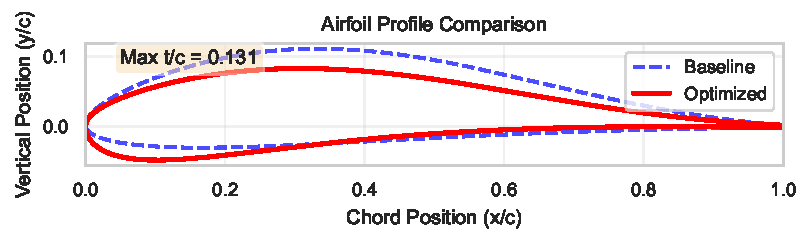
\includegraphics[width=0.8\textwidth]{paper_figures\figure1_airfoil.pdf}
    \caption{Baseline and optimized airfoil profile comparison showing thickness and camber changes.}
    \label{fig:airfoil_comparison}
\end{figure}

% Figure 2: Surface Pressure Distribution
\begin{figure}[htbp]
    \centering
    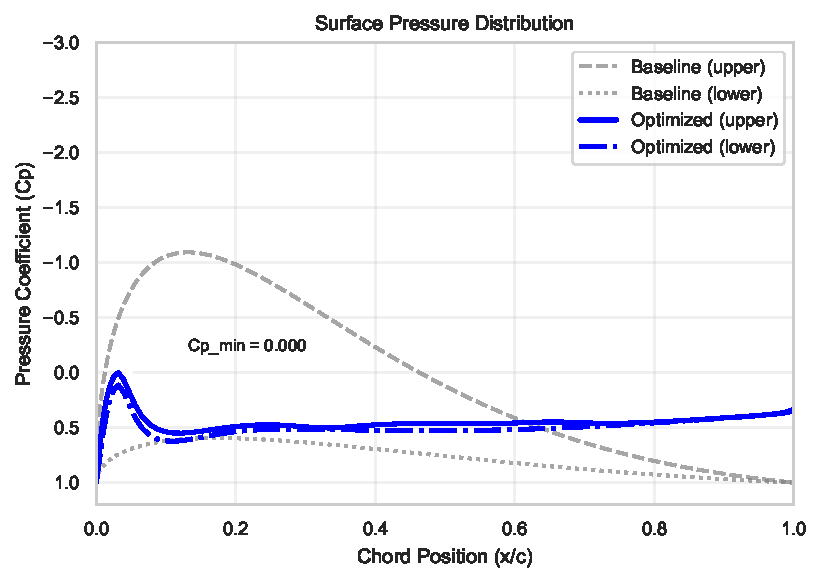
\includegraphics[width=0.8\textwidth]{paper_figures\figure2_pressure.pdf}
    \caption{Surface pressure distribution comparison showing LSB plateau suppression in optimized design.}
    \label{fig:pressure_distribution}
\end{figure}

% Figure 3: Optimization Convergence
\begin{figure}[htbp]
    \centering
    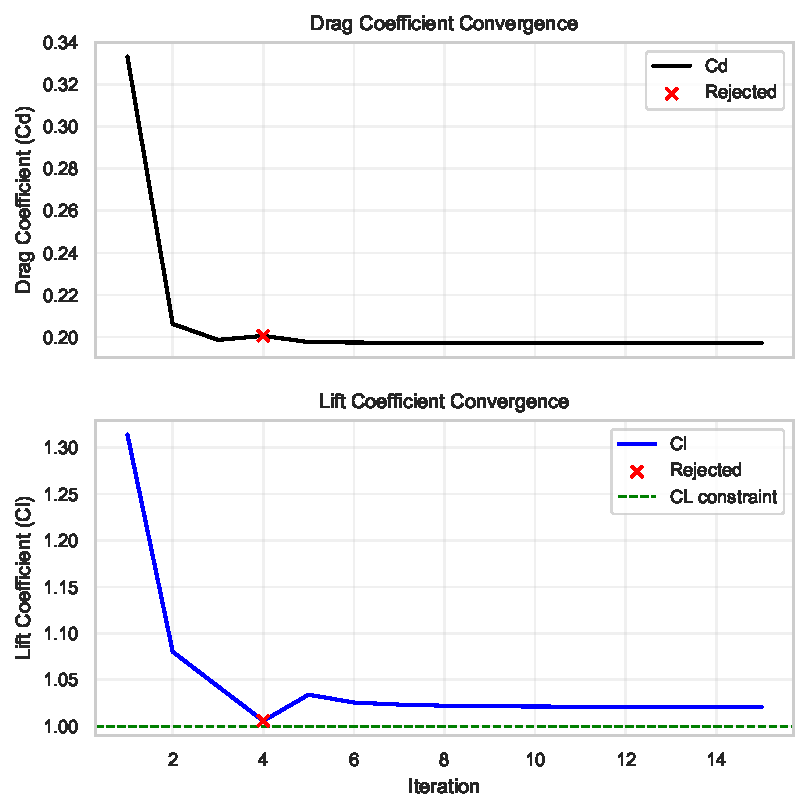
\includegraphics[width=0.8\textwidth]{paper_figures\figure3_convergence.pdf}
    \caption{Optimization convergence history showing drag coefficient reduction and lift constraint satisfaction. Red crosses indicate rejected iterations.}
    \label{fig:convergence}
\end{figure}

% Figure 4: Gradient Decay
\begin{figure}[htbp]
    \centering
    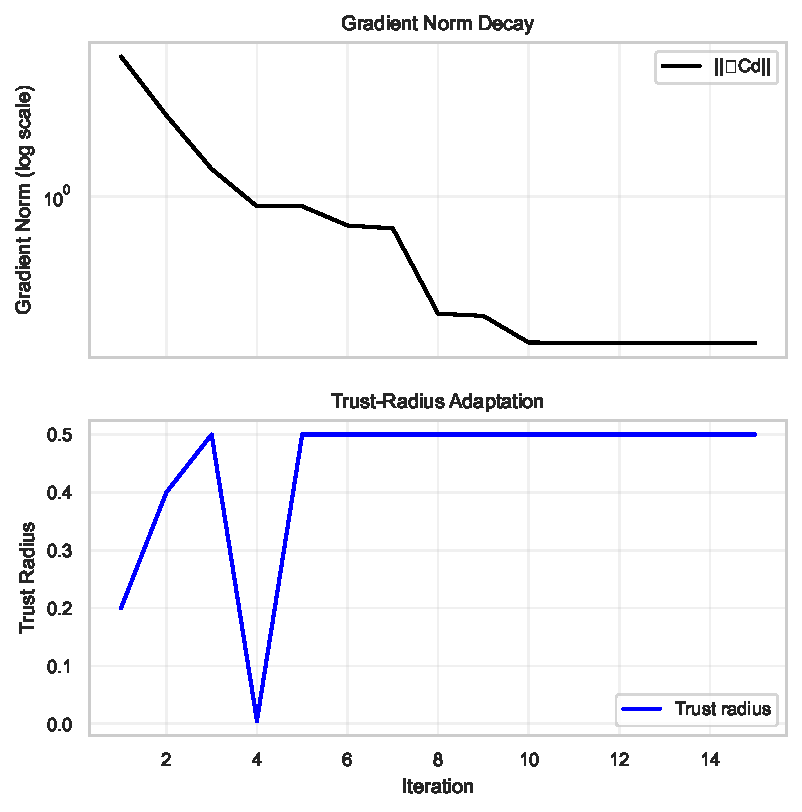
\includegraphics[width=0.8\textwidth]{paper_figures\figure4_gradient.pdf}
    \caption{Gradient norm decay and trust-radius adaptation during optimization, demonstrating algorithm convergence.}
    \label{fig:gradient_decay}
\end{figure}
